%Dies ist die Hauptseite des Dokumentes. Es werden u. a. alle Kapitel,
%Einstellung im Header eingebunden.  Veränderungen müssen in folgenden Dateien
%vorgenommen werden:
      %- Layout.tex
      %- newComments.tex
      %- Titelseite
      %- Versionsübersicht
      %- einzelne Kapitel (evtl. erweitern)


% Definition von globalen Parametern, die derzeit auf der Titelseite und in der
% Kopfzeile verwendet werden. Der in <> gesetzte Text ist zu verändern.

\newcommand{\praktikumTitel}{Ingenieursmäßige Konstruktion, Simulation und Visualisierung von Achterbahnen }
\newcommand{\projektTitel}{Achterbahnsimulator}


%Hier sind alle Einstellungen enthalten, die sich auf das Seiten- und
%Dokumentenlayout beziehen

\documentclass[
  11pt,                % Schriftgröße
  DIV12,
  german,              % für Umlaute, Silbentrennung etc.
  oneside,             % einseitiges Dokument
  titlepage,           % es wird eine Titelseite verwendet
  halfparskip,         % Abstand zwischen Absätzen (halbe Zeile)
  normalheadings,      % Größe der Überschriften verkleinern
  tablecaptionabove,   % Beschriftung von Tabellen unterhalb ausgeben
  final                % Status des Dokuments (final/draft)
]{scrreprt}            %


%------Ändern von Schriftschnitten - (Muss ganz am Anfang stehen !) ------------
\usepackage{fix-cm}

%------Umlaute -----------------------------------------------------------------
%   Umlaute/Sonderzeichen wie äüöß können direkt im Quelltext verwenden werden.
%    Erlaubt automatische Trennung von Worten mit Umlauten.
\usepackage[T1]{fontenc}
\usepackage[utf8]{inputenc}

%------Anpassung der Landessprache----------------------------------------------
\usepackage{ngerman}

%------Einfache Definition der Zeilenabstände und Seitenränder------------------
\usepackage{geometry}
\usepackage{setspace}

%------Schriftgrößenanpassung von einzelnen Textpassagen------------------------
\usepackage{relsize}

%------Trennlinien in Kopf- und Fusszeile
\usepackage[headsepline, footsepline, ilines]{scrpage2}

%------Grafiken-----------------------------------------------------------------
\usepackage{graphicx}

%------Packet zum Sperren, Unterstreichen und Hervorheben von Texten------------
\usepackage{soul}

%------ergänzende Schriftart----------------------------------------------------
\usepackage{helvet}

%------Lange Tabellen-----------------------------------------------------------
\usepackage{longtable}
\usepackage{array}
\usepackage{ragged2e}
\usepackage{lscape}

%------PDF-Optionen-------------------------------------------------------------
\usepackage[
  bookmarks,
  bookmarksopen=true,
  colorlinks=true,
  linkcolor=black,        % einfache interne Verknüpfungen
  anchorcolor=black,      % Ankertext
  citecolor=black,        % Verweise auf Literaturverzeichniseinträge im Text
  filecolor=black,        % Verknüpfungen, die lokale Dateien öffnen
  menucolor=black,        % Acrobat-Menüpunkte
  urlcolor=black,         % Farbe für URL-Links
  backref,                % Zurücktext nach jedem Bibliografie-Eintrag als
                          % Liste von Überschriftsnummern
  pagebackref,            % Zurücktext nach jedem Bibliografie-Eintrag als
                          % Liste von Seitenzahlen
  plainpages=false,       % zur korrekten Erstellung der Bookmarks
  pdfpagelabels,          % zur korrekten Erstellung der Bookmarks
  hypertexnames=false,    % zur korrekten Erstellung der Bookmarks
  linktocpage             % Seitenzahlen anstatt Text im Inhaltsverzeichnis
                          % verlinken
  ]{hyperref}



      % enthält eingebundene Packete

%------Seitenränder-------------------------------------------------------------
\geometry{verbose,                     % zeigt die eingestellten Parameter beim
                                       % Latexlauf an
      paper=a4paper,                   % Papierformat
      top=25mm,                        % Rand oben
      left=25mm,                       % Rand links
      right=25mm,                      % Rand rechts
      bottom=45mm,                     % Rand unten
      pdftex                           % schreibt das Papierformat in die
                                       % Ausgabe damit Ausgabeprogramm
                                       % Papiergröße erkennt
  }

%Seitenlayout
\onehalfspace        % 1,5-facher Abstand

%------Kopf- und Fußzeilen -----------------------------------------------------
\pagestyle{scrheadings}

%------Kopf- und Fußzeile auch auf Kapitelanfangsseiten ------------------------
\renewcommand*{\chapterpagestyle}{scrheadings}

%------Schriftform der Kopfzeile -----------------------------------------------
\renewcommand{\headfont}{\normalfont}

%------Kopfzeile----------------------------------------------------------------
\setlength{\headheight}{21mm}        % Höhe der Kopfzeile
\ihead{\large{\textsc{\praktikumTitel}}\\    % Text in der linken Box
       \small{\projektTitel}}
\chead{}                             % Text in der mittleren Box

%----Fusszeile
\cfoot{}                             % Text in mittlerer Box
\ofoot{\pagemark}                    % Seitenzahl in rechter Box

           % Diese Datei enthält alle
                                           % Layouteinstellungen

%------Beginn des Gesamtdokumentes----------------------------------------------
\begin{document}

%------Eingebundene Seiten, Verzeichnisse bzw. Kapitel--------------------------
% Dies ist die Titelseite des Pflichtenhefts.
% Die in "<...>" sind zu ersetzen
% Die Ausgabe darf 1 Seite nicht überschreiten, also ggf. Abstände anpassen
% Die Angabe in [...] gibt den Abstand nach der entsprechenden Zeile an.


%----Stil dieser Seite----------------------------------------------------------
\thispagestyle{plain}      % Kopfzeile bleibt leer

%----Beginn der Titelseite------------------------------------------------------
\begin{titlepage}

%----zentrierte Ausrichtung über die gesamte Seite----------------------------
\begin{center}

%----Titel des Praktikum (\praktikumTitel in newComments zu verändern)--------
{\relsize{4}{\textbf{\textsc{\praktikumTitel}}}}\\[5ex]

%----Titel des Teilprojektes (\projektTitel in newComments verändern)---------
{\relsize{3}{\textbf{\textsc{\projektTitel}}}}\\[5ex]

Software-Entwicklungspraktikum (SEP)\\
Sommersemester 2011\\[6ex]

{\relsize{3}\so{\textbf{Pflichtenheft}}}\\[5ex]

%----eingebundenes Logo der TU--------------------------------------------------

\includegraphics[scale=0.8]{bilder/carolo.jpg}\\[5ex]

%----Daten des Auftraggebers
Auftraggeber\\
Technische Universität Braunschweig\\
Institut für Wissenschaftliches Rechnen\\
Prof. Hermann G. Matthies, PhD\\
<Straße und Hausnummer>\\
D-38092 Braunschweig\\[2ex]
Betreuer: Elmar Zander\\[5ex]

% ----Tabelle der Praktikumsteilnehmer------------------------------------------
Auftragnehmer: <überzählige Zeilen löschen>\\

\begin{tabular}{l<{\hspace{20mm}} l<{\hspace{30mm}}}\\
  Name                   &   E-Mail-Adresse\\      % Zeilenüberschift

  \hline                    % Linie unterhalb der Zeilenüberschrift

  %----Nachfolgend alle Namen und E-Mail-Adressen der Teilnehmer einfügen
  Matthias Überheide> &  m.ueberheide@tu-bs.de\\
  Christian Mangelsdorf &  ch.mangelsdorf@googlemail.com\\
	Daniel Bahn & danielbahn@arcor.de\\
	Simon Hahne & MrSimWob@aol.com\\
	Robin Hofmann & hofmann.robin@web.de\\
	Marco Melzer & marco.melzer@tu-braunschweig.de\\
	Konstantin Birker & k.birker@tu-braunscheig.de\\

\end{tabular}\\[2ex]

Braunschweig, \today

\end{center}
\end{titlepage}
                       % Titelseite

%Diese Datei dient der Versionskontrolle. Sie ist vollständig zu bearbeiten.

%----Überschrift------------------------------------------------------------
{\relsize{2}\textbf{Versionsübersicht}}\\[2ex]

%----Start der Tabelle------------------------------------------------------
\begin{longtable}{|m{1.78cm}|m{1.59cm}|m{2.86cm}|m{1.9cm}|m{5.25cm}|}

  \hline                                              % Linie oberhalb

  %----Spaltenüberschriften------------------------------------------------
  \textbf{Version}  &    \textbf{Datum}  &    \textbf{Autor}  &
  \textbf{Status}   &    \textbf{Kommentar}       \\  %Spaltenüberschrift
  \hline                                              % Gitterlinie

  %----die nachfolgeden beiden Zeilen so oft wiederholen und die ... mit den
  %    entsprechenden Daten zu füllen wie erforderlich
  0.1&02.05.2011&Christian Mangelsdorf&in Bearbeitung&Initialisierung\\
  \hline
  0.2&04.05.2011&Simon Hahne, Robin Hoffman, Christian Mangelsdorf&in Bearbeitung&Komponentenspezifiktion\\
  \hline
  0.3&06.05.2011&Matthias Überheide&in Bearbeitung&Vorbereitung Funktionsanalyse\\
  \hline
  0.4&08.05.2011&Matthias Überheide, Daniel Bahn, Konstantin Birker, Robin Hoffman, Simon Hahne, Christian Mangelsdorf&in Bearbeitung&Sequenzdiagramme und Statcharts\\
  \hline
  0.5&09.05.2011&Matthias Überheide, Daniel Bahn, Robin Hoffman, Simon Hahne, Christian Mangelsdorf&in Bearbeitung&Änderungen gemäß Besprechung\\
  \hline
  0.6&10.05.2011&Matthias Überheide, Christian Mangelsdorf&in Bearbeitung&Schnittstellenspezifikation\\
  \hline
  0.7&11.05.2011&Matthias Überheide, Daniel Bahn, Konstantin Birker, Robin Hoffman, Simon Hahne, Christian Mangelsdorf, Marco Melzzer&abgenommen&Korrekturen\\
  \hline
  %...    &    ...    &    ...    &    ...    &    ...\\       % Eintrag in Zeile
  \hline                                              % Gitterlinie unten

%----Ende der Tabelle------------------------------------------------------
\end{longtable}

%Status: "`in Bearbeitung"' oder "`abgenommen"'
%Kommentar: hier eintragen, was geändert bzw. ergänzt wurde


%Hinweis zum Template:
%Dieses Template enthält Hinweise, die alle kursiv geschrieben sind. Alles
%Kursivgeschriebene ist selbstverständlich bei Abgabe zu entfernen sind.
%Angaben in <\ldots> sind mit dem entsprechendem Text zu füllen.  Überzählige
%Kapitel, d. h. Kapitel, die nicht bearbeitet werden müssen, da sie nicht der
%Aufgabenstellung entsprechen, bitte entfernen.

%Aufgabe des Grobentwurfs: Aufgabe dieses Dokumentes ist es, die Architektur des
%Systems zu beschreiben und die daraus resultierenden Pakete durch die
%Definition von Schnittstellen zu Komponenten auszubauen.
        % Versionsübersicht

\tableofcontents                           % Inhaltsverzeichnis wird automatisch
                                           % generiert
\listoffigures                             % ebenso das Abbildungsverzeichnis

%----Kapitel des Feinentwurfs, die mit Inhalt zu füllen sind--------------------
% Kapitel 1
% Die Unterkapitel können auch in separaten Dateien stehen,
% die dann mit dem \include-Befehl eingebunden werden.
%-------------------------------------------------------------------------------

\chapter{Zielbestimmung}
Ziel dieses Projektes ist die Erstellung eines Simulators zur 3D-Visualisierung von Achterbahnfahrten. Der Simulator soll einem Ingenieur den schnellen Überblick über den Fahrtverlauf aus Sicht des Fahrgastes ermöglich. Neben der räumlichen Orientierung interessieren auch die Beschleunigungen, die auf die Passagiere während der Fahrt einwirken. Der Simulator wird auch zum Zwecke der Präsentationen beispielsweise gegenüber dem Auftraggeber zum Einsatz kommen.

\section{Musskriterien}
Die primäre Aufgabe des Simulators besteht in der physikalisch korrekten Wiedergabe des Fahrverhaltens der Achterbahn aus der Perspektive eines Fahrgasts. Die Berechnung und Darstellung der Fahrt muss in Echtzeit erfolgen.

Zur 3D-Visualisierung der Achterbahn gehört zwingend die Darstellung eines ebenen Bodens als Grundfläche, zweier parallel verlaufender Schienen und mindestens zweier Querbalken pro Streckenabschnitt.

Zusätzlich ist zwingend eine 2D-Visualisierung der Beschleunigungen erforderlich, die während der Fahrt auf die Insassen des Achterbahnwaagen einwirken.

Das Programm benötigt eine Oberfläche zum Einlesen der Achterbahn-Spezfikationen und zum Einstellen der Programmoptionen.

\section{Wunschkriterien}

Es bestehen verschiedene Verbessungsmöglichkeiten an der physikalischen Simulation der Achterbahn. Durch Berücksichtigung der Luft- und Bahnreibung kann der Energieverlust beim Fahrbetrieb erfasst werden, der für einen Dauerbetrieb durch zusätzlichen Antrieb ausgeglichen werden müsste. Entsprechendes gilt für die Berücksichtigung der Bremsvorgänge. Eine Berücksichtigung der Beschleunigungskäfte durch außeraxiale Massen wie Wagen und Passagiere ist denkbar.

Um eine für Präsentationen attraktive 3D-Visualisierung der Achterbahnen umzusetzen, sind mehrere Ergänzungen wünschenswert. Neben den Schienen und den Querbalken sollten auch die Stützbalken für die Streckenabschnitte dargestellt werden. Eine Darstellung der Umgebung mit Gebäuden, Bepflanzung und Himmel verleiht dem Zuschauer der Simulation eine bessere Orientierungsmöglichkeit. Für einen realistischen Boden sollten Unebenheiten zulässig sein.

Je nach Rechenleistung wäre neben einer Darstellung der Achterbahnfahrt aus der Passagierperspektive auch eine Außenperspektive mit verstellbarer Kamera wünschenswert. In diesem Fall müsste zwingend eine Modellierung des Achterbahnwagens erfolgen.

Eine Zeitrafferfunktion mit der Möglichkeit zum Vor- und Zurückspulen würde die Untersuchung bestimmter Streckenabschnitte erleichtern.

Wünschenwert ist auch Aufnahmefunktion für Einzelbilder oder Filme, die in gängigen Dateiformaten exportiert und damit auch außerhalb des Simulators weiterverarbeitet werden könnten.

\section{Abgrenzungskriterien}
Der Simulator besitzt keine eigenständige Funktionalität zum Erstellen oder Ändern der Achterbahnen. Für diese Aufgaben muss auf die Programmkomponenten aus dem Teilprojekt "Achterbahneditor" zurückgegriffen werden.

Die statischen und dynamischen Belastungen auf das Achterbahntragwerk werden nicht simuliert. Insbesondere wird die Tragfähigkeit des Gerüstes nicht geprüft.

Mögliche Einflüsse der Umgebung auf die Achterbahn werden nicht berücksichtigt. Beispielsweise werden Einschränkungen der Sicht durch Regen- oder Dunst nicht dargestellt. Die Auswirkungen des Windes auf das Fahrverhalten der Achterbahn werden ignoriert.

Eine Simulation der Passagierbeförderung mit Ein- und Ausstieg findet nicht statt. Die Wirksamkeit von Sicherungsmaßnahmen wie Gurte oder Haltebügel wird nicht untersucht.             % Kapitel 1
% Kapitel 2 mit den entsprechenden Unterkapiteln
% Die Unterkapitel können auch in separaten Dateien stehen,
% die dann mit dem \include-Befehl eingebunden werden.
%------------------------------------------------------------------------------------

\chapter {Produkteinsatz}

Die Simulation soll dem technischen Entwickler der Achterbahnen als Visualisierungswerkzeug für die physikalischen Gegebenheiten
dienen. Dadurch können durchgeführte Änderungen im Editor sofort optisch dargestellt und interpretiert werden.
Desweiteren soll die Simulation auch als Präsentationswerkzeug dienen.

\section {Anwendungsbereiche}
Kontruktionsbereich, technischer Entwicklungsbereich

\section {Zielgruppen}
Ingenieure, Präsentationspublikum

\section {Betriebsbedingungen}
Es handelt sich um eine Einzelplatzanwendung, die an einem Bürorechner oder Notebook betrieben werden kann.
Die Anwendung sollte mit einer 2 Jahre alten Grafikkarte mit 3D Beschleunigung lauffähig sein.
Der Simulator soll mit dem existierenden Editor zusammenspielen und auch gleichzeitig betrieben werden können.            % Kapitel 2
% Kapitel 3
%-------------------------------------------------------------------------------
\chapter{Produktübersicht}

\begin{center}
%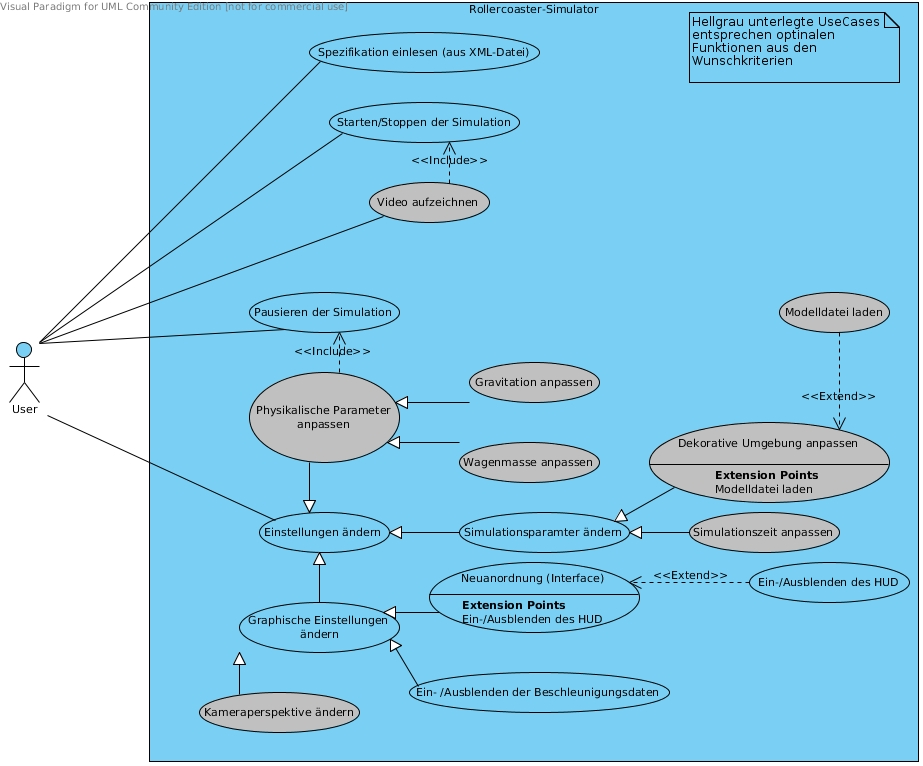
\includegraphics[scale=0.5]{bilder/usecase1.jpg}
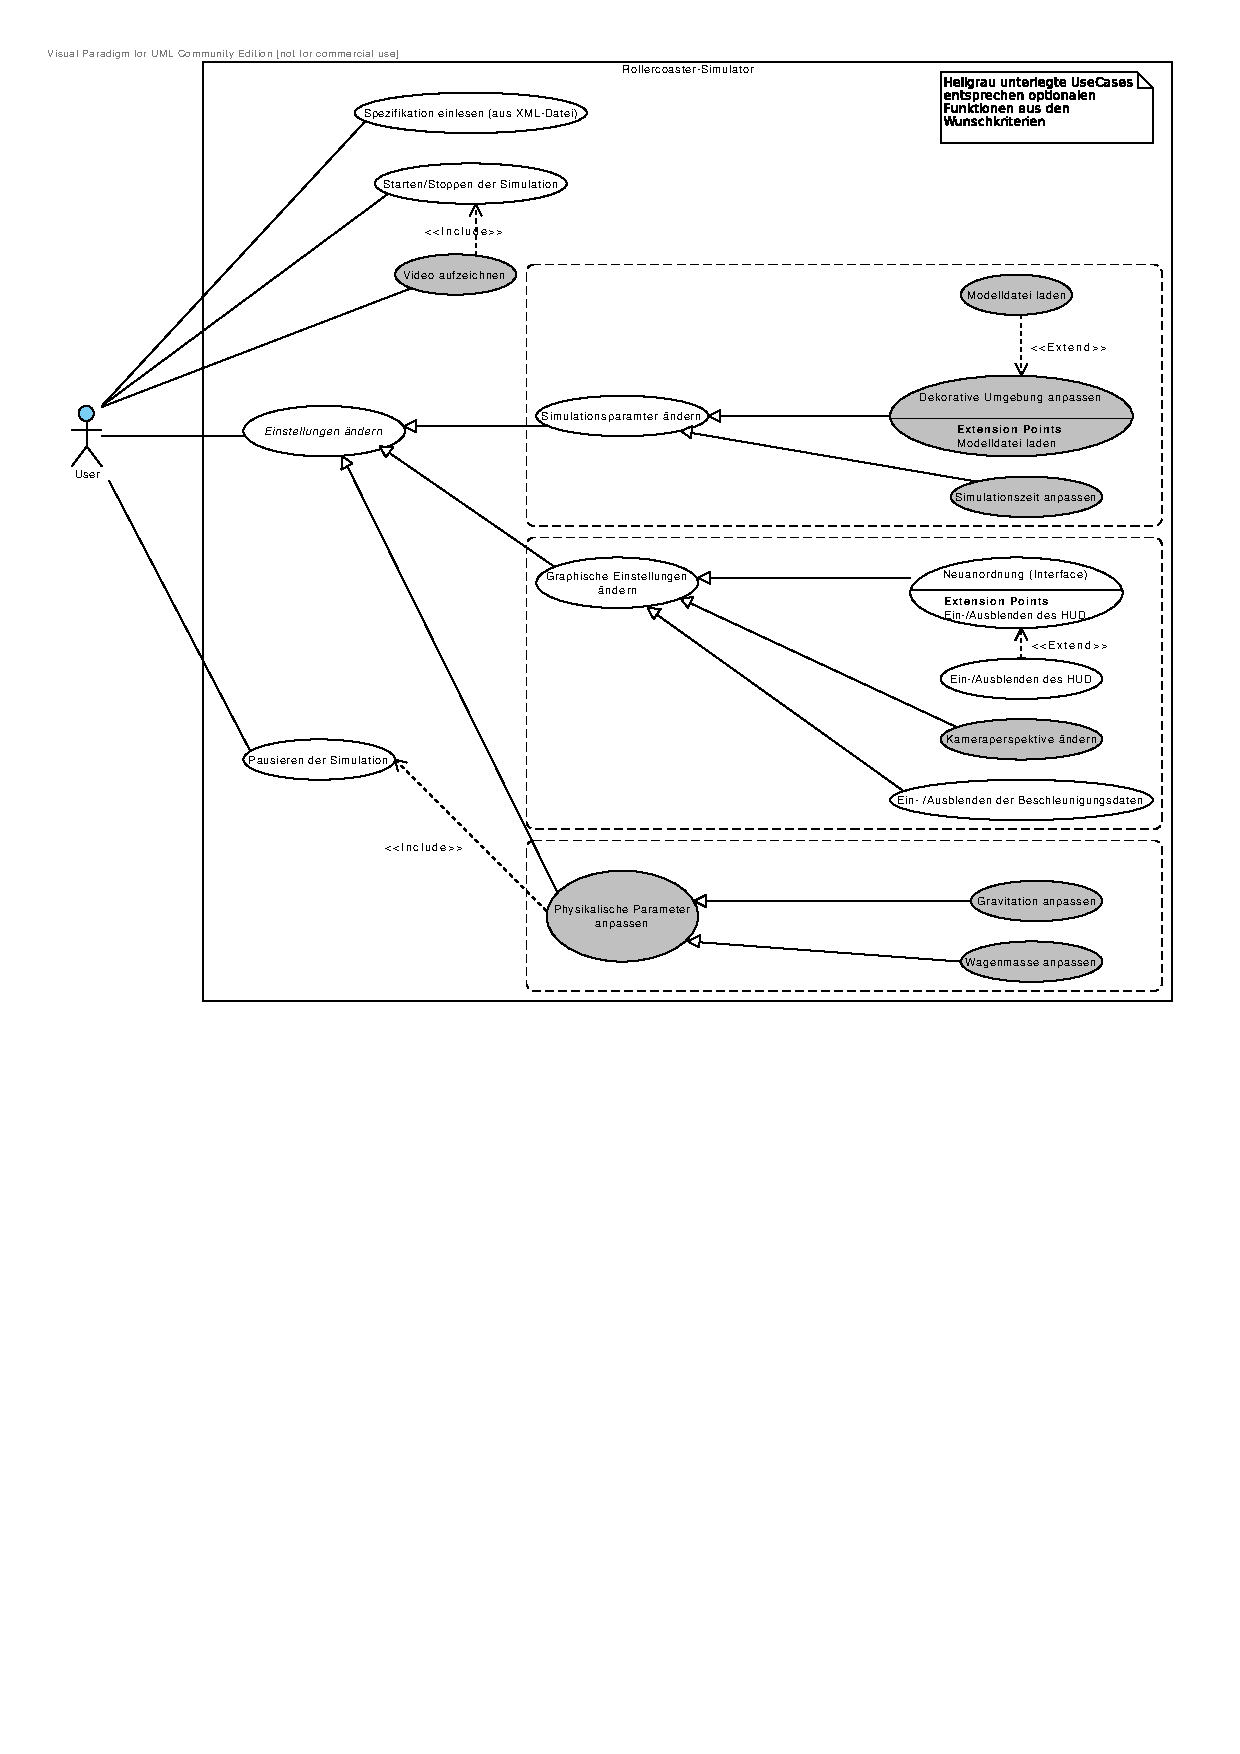
\includegraphics[scale=0.85]{bilder/usecase1.pdf}
\end{center}         % Kapitel 3
% Kapitel 4
%-------------------------------------------------------------------------------

\chapter{Produktfunktionen}

Im Nachfolgenden werden die Produktfunktionen näher beschrieben. Um optionale Funktionen zu Kennzeichnen sind die entsprechenden Prozesse mit einem zusätzlichen o im Kürzel bezeichnet.
\\ \\ 

/F100/\\
\textbf{Geschäftsprozess:} Spezifikation einlesen \\
\textbf{Ziel:} Ein Dateipfad wird angegeben und die neue Bahn der zu simulierenden Achterbahn wird der XML-Datei in allen Parametern entnommen. \\
\textbf{Vorbedingung:} Ein valider Dateiname wurde übergeben; Die Simulation ist gestopt oder pausiert \\
\textbf{Nachbedingung Erfolg:} Die neue Bahn steht in allen Parametern dem Simulator im Speicher zur Verfügung. Der Ausgangszustand für eine Simulation wird hergestellt. \\
\textbf{Nachbedingung Fehlschlag:} Der Zustand vor dem Prozess ist wiederhergestellt. \\
\textbf{Akteure:} User \\
\textbf{Auslösendes Ereignis:} Userinteraktion \\
\textbf{Beschreibung:} \\
1 Der User wählt über einen Dateidialog eine XML Datei aus. \\
2 Das Programm interpretiert diese und ließt die enthaltenen Paramter ein. \\
- ein Syntaxcheck wird durchgeführt und ggf eine Fehlermeldung angezeigt\\
3 Die Daten werden in die Objekte des Simulators eingegeben. Fehlende Einträge werden soweit möglich mit Defaultwerten belegt.\\
\textbf{Erweiterungen:}\\
\textbf{Alternativen:}\\
\\
/F200/\\
\textbf{Geschäftsprozess:} Starten/Stoppen der Simulation\\
\textbf{Ziel:} Die Simulation der Achterbahn wird gestartet oder gestopt\\
\textbf{Vorbedingung:} Eine Achterbahnstrecke ist geladen\\
\textbf{Nachbedingung Erfolg:} Der Status wird gewechselt (von gestartet auf gestopt bzw umgekehrt)\\
\textbf{Nachbedingung Fehlschlag:} Fehlermeldung; Simulation gestopt\\
\textbf{Akteure:} User\\
\textbf{Auslösendes Ereignis:} Userinteraktion\\
\textbf{Beschreibung:} Der User interagiert über eine Schaltfläche die je nach aktuellem Status für die jeweilige Umschaltfunktion steht und verändert damit den Simulationsstatus.\\
Das Stoppen führt zum Abbau von temporären Ergebnissen. Ein Fortsetzen der Simulation ist nicht mehr möglich (aber ein Neustart am Streckenanfang)\\
\textbf{Erweiterungen:}\\
\textbf{Alternativen:}\\
\\
/F300/\\
\textbf{Geschäftsprozess:} Pausieren der Simulation\\
\textbf{Ziel:} Die Simulation wird pausiert kann jedoch zu einem späteren Zeitpunkt wieder fortgesetzt werden.\\
\textbf{Vorbedingung:} Eine Simulation läuft\\
\textbf{Nachbedingung Erfolg:} Die Simulation ist Unterbrochen\\
\textbf{Nachbedingung Fehlschlag:} \\
\textbf{Akteure:} User\\
\textbf{Auslösendes Ereignis:} Userinteraktion\\
\textbf{Beschreibung:} \\
\textbf{Erweiterungen:}\\
\textbf{Alternativen:}\\
\\
/F400o/ \\
\textbf{Geschäftsprozess:} Video aufzeichnen\\
\textbf{Ziel:} Es wird ein Video der Visualisierung mit den aktuell zur Anzeige ausgewählten Informationen erzeugt und auf der Festplatte abgespeichert.\\
\textbf{Vorbedingung:} Eine Simulation ist geladen (und läuft nicht; ggf wird die Simulation gestopt), die gewählte Zieldatei ist noch nicht existent, der Zielort ist beschreibbar\\
\textbf{Nachbedingung Erfolg:} Es existiert eine Videodatei auf der Festplatte die mit einem herkömmlichen Player abspielbar ist.\\
\textbf{Nachbedingung Fehlschlag:} Es existiert eine Datei auf der Festplatte, die die Daten der Aufzeichnung soweit wie möglich erhält.\\
\textbf{Akteure:} User\\
\textbf{Auslösendes Ereignis:} Userinteraktion\\
\textbf{Beschreibung:}  Der User wählt einen Zielort, und zeichnet das Video der Fahrt bis zum Ende der Strecke auf.\\
\textbf{Erweiterungen:}\\ 
\textbf{Alternativen:}\\
\\
/F500/\\
\textbf{Geschäftsprozess:} Einstellungen ändern\\
\textbf{Ziel:} Teile der Einstellungen der Simulationsumgebung werden verändert\\
\textbf{Vorbedingung:} \\
\textbf{Nachbedingung Erfolg:} Die Änderungen in den Einstellungen wurden umgesetzt\\
\textbf{Nachbedingung Fehlschlag:}  Die Änderungen wurden mit einer Fehlermeldung zurückgewiesen\\
\textbf{Akteure:} User\\
\textbf{Auslösendes Ereignis:} Userinteraktion\\
\textbf{Beschreibung:} \\
\textbf{Erweiterungen:}\\
\textbf{Alternativen:}\\
\\
/F510o/\\
\textbf{Geschäftsprozess:} Physikalische Paramter anpassen\\
\textbf{Ziel:} Parameter der Physikalischen Berechnung werden angepasst und verändern damit den Fortlauf der Simulation\\
\textbf{Vorbedingung:} Eine Achterbahn ist geladen\\
\textbf{Nachbedingung Erfolg:} Die Änderungen wurden gespeichert und eine etwaig laufende Simulation pausiert\\
\textbf{Nachbedingung Fehlschlag:}  Die Änderungen wurden mit einer Fehlermeldung zurückgewiesen\\
\textbf{Akteure:} User\\
\textbf{Auslösendes Ereignis:} Userinteraktion\\
\textbf{Beschreibung:} \\
\textbf{Erweiterungen:} Der User kann in einem Dialog gefragt werden ob er wegen der neuen physikalischen Grundlagen die Simulation komplett neustarten möchte\\
\textbf{Alternativen:}\\
\\
/F511o/\\
\textbf{Geschäftsprozess:} Gravitation anpassen\\
\textbf{Ziel:} Für die Simulation wird eine andere wirkende Gravitation in Richtung des Bodens vorausgesetzt. Die Berechnungen ändern sich entsprechend.\\
\textbf{Vorbedingung:} Eine Achterbahn ist geladen\\
\textbf{Nachbedingung Erfolg:} Die Änderungen wurden gespeichert und eine etwaig laufende Simulation pausiert\\
\textbf{Nachbedingung Fehlschlag:}  Die Änderungen wurden mit einer Fehlermeldung zurückgewiesen\\
\textbf{Akteure:} User\\
\textbf{Auslösendes Ereignis:} Userinteraktion\\
\textbf{Beschreibung:} \\
\textbf{Erweiterungen:} Der User kann in einem Dialog gefragt werden ob er wegen der neuen physikalischen Grundlagen die Simulation komplett neustarten möchte\\
\textbf{Alternativen:}\\
\\
/F512o/\\
\textbf{Geschäftsprozess:} Wagenmasse anpassen\\
\textbf{Ziel:} Die Masse des Wagens wir mit dem neuen Wert angenommen und verändert das Simulationsergebnis.\\
\textbf{Vorbedingung:} Eine Achterbahn ist geladen\\
\textbf{Nachbedingung Erfolg:} Die Änderungen wurden gespeichert und eine etwaig laufende Simulation pausiert\\
\textbf{Nachbedingung Fehlschlag:}  Die Änderungen wurden mit einer Fehlermeldung zurückgewiesen\\
\textbf{Akteure:} User\\
\textbf{Auslösendes Ereignis:} Userinteraktion\\
\textbf{Beschreibung:} \\
\textbf{Erweiterungen:} Der User kann in einem Dialog gefragt werden ob er wegen der neuen physikalischen Grundlagen die Simulation komplett neustarten möchte\\
\textbf{Alternativen:}\\
\\
/F520/\\
\textbf{Geschäftsprozess:} Simulationsparameter ändern\\
\textbf{Ziel:} Parameter die den Ablauf der Simulation bestimmen werden verändert und die Simulation wird fortgesetzt\\
\textbf{Vorbedingung:}  \\
\textbf{Nachbedingung Erfolg:} neue Einstellungen übernommen\\
\textbf{Nachbedingung Fehlschlag:} alte Einstellungen bleiben intakt\\
\textbf{Akteure:} User\\
\textbf{Auslösendes Ereignis:} Userinteraktion\\
\textbf{Beschreibung:} \\
\textbf{Erweiterungen:}\\
\textbf{Alternativen:}\\
\\
/F521o/\\
\textbf{Geschäftsprozess:} Dekorative Umgebung anpassen\\
\textbf{Ziel:} Die Dekorative umgebung wird erweitert bzw reduziert.\\
\textbf{Vorbedingung:} \\
\textbf{Nachbedingung Erfolg:} die neuen dekorativen Elemente werden in der Visualisierung angezeigt\\
\textbf{Nachbedingung Fehlschlag:} alte Einstellungen bleiben intakt\\
\textbf{Akteure:} User\\
\textbf{Auslösendes Ereignis:} Userinteraktion\\
\textbf{Beschreibung:} Aus einigen Elementen kann gewählt werden welche zur Anzeige kommen sollen. Bspw können Geländetopologieen oder zusätzliche Stützen aktivierbar sein.\\
\textbf{Erweiterungen:} Eine Modelldatei wird geladen die dann als Dekoelement eingefügt wird.\\
\textbf{Alternativen:}\\
\\
/F522o/\\
\textbf{Geschäftsprozess:} Simulatioszeit anpassen\\
\textbf{Ziel:} Die Geschwindigkeit der Simulation wird verändert.\\
\textbf{Vorbedingung:} \\
\textbf{Nachbedingung Erfolg:} neue Geschwindigkeitseinstellung übernommen\\
\textbf{Nachbedingung Fehlschlag:} alte Geschwindigkeitseinstellung bleiben intakt\\
\textbf{Akteure:} User\\
\textbf{Auslösendes Ereignis:} Userinteraktion\\
\textbf{Beschreibung:} Die Zeitschritte mit denen die Physik berechnet wird, wird manipuliert\\
\textbf{Erweiterungen:}\\
\textbf{Alternativen:}\\
\\
/F530/\\
\textbf{Geschäftsprozess:}  Graphische Einstellungen ändern\\
\textbf{Ziel:}  Das graphische Erscheinungsbild des Programms wird verändert\\
\textbf{Vorbedingung:} \\
\textbf{Nachbedingung Erfolg:} Das Erscheinungsbild wurden nach den wünschen des Users angepasst\\
\textbf{Nachbedingung Fehlschlag:} Das alte Erscheinungsbild ist in Kraft\\
\textbf{Akteure:} User\\
\textbf{Auslösendes Ereignis:} Userinteraktion\\
\textbf{Beschreibung:} \\
\textbf{Erweiterungen:}\\
\textbf{Alternativen:}\\
\\
/F531/\\
\textbf{Geschäftsprozess:}  Neuanordnung (Interface)\\
\textbf{Ziel:}  Das graphische Erscheinungsbild der Programmoberfläche wird verändert\\
\textbf{Vorbedingung:} \\
\textbf{Nachbedingung Erfolg:} Das Erscheinungsbild wurden nach den wünschen des Users angepasst\\
\textbf{Nachbedingung Fehlschlag:} Das alte Erscheinungsbild ist in Kraft\\
\textbf{Akteure:} User\\
\textbf{Auslösendes Ereignis:} Userinteraktion\\
\textbf{Beschreibung:} Das Interface des Programms wird nach den Wünschen des Users verschoben\\
\textbf{Erweiterungen:} Aus/Einblenden eines HUD\\
\textbf{Alternativen:}\\
\\
/F532/\\
\textbf{Geschäftsprozess:}  Ein/Ausblenden von Beschleunigungsdaten\\
\textbf{Ziel:}  Das Fenster mit den Graphen der physikalischen Werte wird ein bzw ausgeblendet\\
\textbf{Vorbedingung:} \\
\textbf{Nachbedingung Erfolg:} Das Graphenfenster ist ein- bzw ausgeblendet\\
\textbf{Nachbedingung Fehlschlag:}\\ 
\textbf{Akteure:} User\\
\textbf{Auslösendes Ereignis:} Userinteraktion\\
\textbf{Beschreibung:} \\
\textbf{Erweiterungen:}\\
\textbf{Alternativen:}\\
\\
/F533o/\\
\textbf{Geschäftsprozess:}  Kameraperspektive ändern\\
\textbf{Ziel:}  Die perspektive der Kamera ändert sich zwischen unterscheidlichen Modi\\
\textbf{Vorbedingung:} \\
\textbf{Nachbedingung Erfolg:} Eine neue Kameraperspektive ist aktiv aus der die Bilder gerendert werden\\
\textbf{Nachbedingung Fehlschlag:} Das alte Perspektive ist in Kraft\\
\textbf{Akteure:} User\\
\textbf{Auslösendes Ereignis:} Userinteraktion\\
\textbf{Beschreibung:} Durch entsprechende Interaktion kann zwischen vorgefertigten Perspektiven umgeschaltet werden, sodass die Fahrt auch aus anderen Blickwinkeln betrachtet werden kann\\
\textbf{Erweiterungen:}\\
\textbf{Alternativen:}\\
\\
% die restlichen <1000 ggf reservieren für weitere Interfacefunktionen
/F1000/\\
\textbf{Geschäftsprozess:} Warnung vor hoher Beschleunigung\\
\textbf{Ziel:} Der User wird von der Überschreitung von gefährlichen Beschleunigungsgrenzen in Kenntnis gesetzt\\
\textbf{Vorbedingung:} Eine Fahrt wird simuliert\\
\textbf{Nachbedingung Erfolg:} Eine Nachricht wurde ausgegeben\\
\textbf{Nachbedingung Fehlschlag:} \\
\textbf{Akteure:} Simulation\\
\textbf{Auslösendes Ereignis:} Überschreitung von Grenzwerten\\
\textbf{Beschreibung:} Bei der überschreitung von gefährlichen Grenzwerten bei den Beschleunigungen warnt das Programm mit entsprechenden Effekten bzw einer Nachricht\\
\textbf{Erweiterungen:}\\
\textbf{Alternativen:}\\
         % Kapitel 4
% Kapitel 5
%------------------------------------------------------------------------------------------

\chapter{Produktdaten}
5  Produktdaten
Die langfristig zu speichernden Daten sind aus Benutzersicht detaillierter zu
beschreiben. Dabei bietet sich eine formale Beschreibung (z. B. in Form eines
Data Dictionary) an, um eine größere Präzisierung zu erreichen.

Bitte die Darstellung gemäß Beispiel verwenden:\\
-  /D10/: fortlaufende Nummerierung der Daten\\
-  /LD10/: vordefinierte Daten aus dem Lastenheft (falls vorhanden).\\

Beispiel: Lagerdaten\\
/D10/ (/LD10/) Daten der Lagerplätze (max. 5.000):\\
-  Modulnummer,\\
-  Regalseite,\\
-  Regalspalte,\\
-  Regalzeile,\\
-  Fachhöhe,\\
-  Platzsperre (0 = nicht gesperrt, 1 = gesperrt für Einlagerung, 2 = gesperrt
   für Auslagerung, 3 = gesperrt für alle Zugriffe),\\
-  Reifenstatus (0 = frei,1 = reserviert für Einlagerung, 2= belegt, 3 =
   reserviert für Auslagerung),\\
-  Reifenseriennummer.\\

/D40/ (/LD40/) Daten der Module (max. 20):\\
-  Modulnummer,\\
-  Sperrkennzeichen (0 = nicht gesperrt, 1 = gesperrt für Einlagerung, 2 =
   gesperrt für Auslagerung, 3 = gesperrt für alle Zugriffe),\\
-  maximale Kapazität,\\
-  freie Kapazität,\\
-  belegte Plätze (ergibt sich aus Status und Zahl der zugeordneten
   Lagerplätze, wird aus Geschwindigkeitsgründen allerdings redundant
   mitgeführt).

              % Kapitel 4
% Kapitel 6 
%-------------------------------------------------------------------------------

\chapter{Nichtfunktionale Anforderungen}


%----Start der Tabelle------------------------------------------------------
\begin{tabular}{|c|c|c|c|c|}
  \hline                                              % Linie oberhalb

  %----Spaltenüberschriften------------------------------------------------
  \textbf{Produktqualität}  & \textbf{sehr gut}  &    \textbf{gut}  &
  \textbf{normal}           & \textbf{nicht relevant}  \\  %Spaltenüberschrift
  \hline                                              % Gitterlinie

  %----die nachfolgeden beiden Zeilen so oft wiederholen und die ... mit den
  %    entsprechenden Daten zu füllen wie erforderlich
  \textbf{Funktionalität}  &&&&\\        % Eintrag in Zeile
  \hline
Angemessenheit&&x&&\\
\hline
Richtigkeit&x&&&\\
\hline
Interoperabilität&&&x&\\
\hline
Ordnungsmäßgkeit&&&x&\\
\hline
\textbf{Sicherheit}&&&&\\
\hline
Zuverlässigkeit&&x&&\\
\hline
Reife&&x&&\\
\hline
Fehlertoleranz&&&x&\\
\hline
Wiederherstellbarkeit&&&x&\\
\hline
\textbf{Benutzbarkeit}&&&&\\
\hline
Verständlichkeit&&&x&\\
\hline
Erlernbarkeit&&x&&\\
\hline
Bedienbarkeit&x&&&\\
\hline
Effizienz&x&&&\\
\hline
Zeitverhalten&x&&&\\
\hline
Verbrauchsverhalten&&&x&\\
\hline
\textbf{Änderbarkeit}&&&&\\
\hline
Analysierbarkeit&&&x&\\
\hline
Modifizierbarkeit&&x&&\\
\hline
Stabilität&&&x&\\
\hline
Prüfbarkeit&&x&&\\
\hline
Übertragbarkeit&&&&\\
\hline
Anpassbarkeit&&&&x\\
\hline
Installierbarkeit&&x&&\\
\hline
Konformität&&&x&\\
\hline
Austauschbarkeit&&&&x\\
\hline
%----Ende der Tabelle------------------------------------------------------
\end{tabular}

\begin{itemize}

\item  /Q10/ Das Produkt soll in Java geschrieben sein.
\item  /Q20/ Das Produkt muss unter Linux laufen.
\item  /Q30/ Das Produkt soll auf einem Computer mit OpenGL-fähiger Grafikkarte laufen.
\item  /Q40/ Die Simulation soll in Echtzeit berechnet werden.
\item  /Q50/ Die Simulation soll stabil laufen, soweit es die 3D-Grafikkartentreiber erlauben.

\end{itemize}
        % Kapitel 4
% Kapitel 8
%-------------------------------------------------------------------------------

\chapter{Benutzeroberfläche}
%%Einleitung
Es sind zwei unterschiedliche Oberflächen geplant, je nach Zustand des Programms. Die Erste zeigt nach dem Laden der Konstruktionsdatei eine grafische Übersicht der Konstruktion, sowie Informationen zu der geladenen Datei. Die Zweite und wichtigere die Simulation und die dazugehörigen Messdaten. Die Unterteilung des Bildschirms ist in drei Bereiche vorgesehen, die je nach Programmzustand (Simulation oder Vorschau) unterschiedliche Informationen oder Einstellmöglichkeiten bieten.




%%Bild
\begin{figure}[!h]%
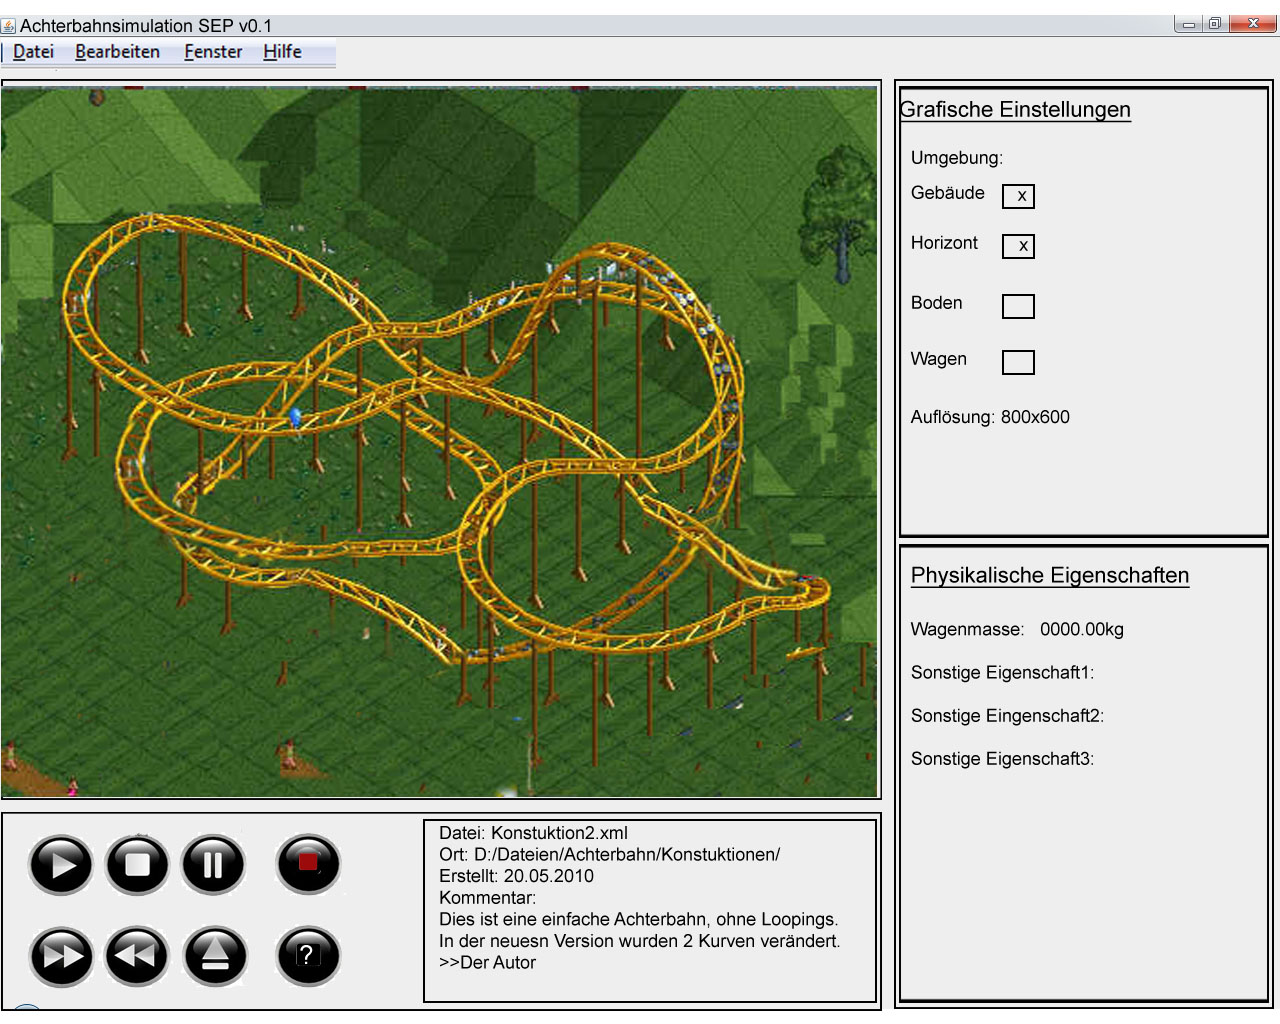
\includegraphics[width=0.8\linewidth]{./bilder/GUI_v3.jpg}%
\caption{Vorschau}%
\label{Vorschau}%
\end{figure}

%%Beschreibung des Vorschaubiles
\section*{Vorschau}
Die Oberfläche ist in drei Bereiche der gleichen Größe im Simulationsbildschirm aufgeteilt. Im Mittleren wird eine Übersicht über die geladene Konstruktion gezeigt, auf der rechten Seite befinden sich Einstellungen zur Grafik und physikalischen Werten und im unteren mittleren Bereich werden Informationen über die Datei bereitgestellt.


%%Bild
\begin{figure}[!h]%
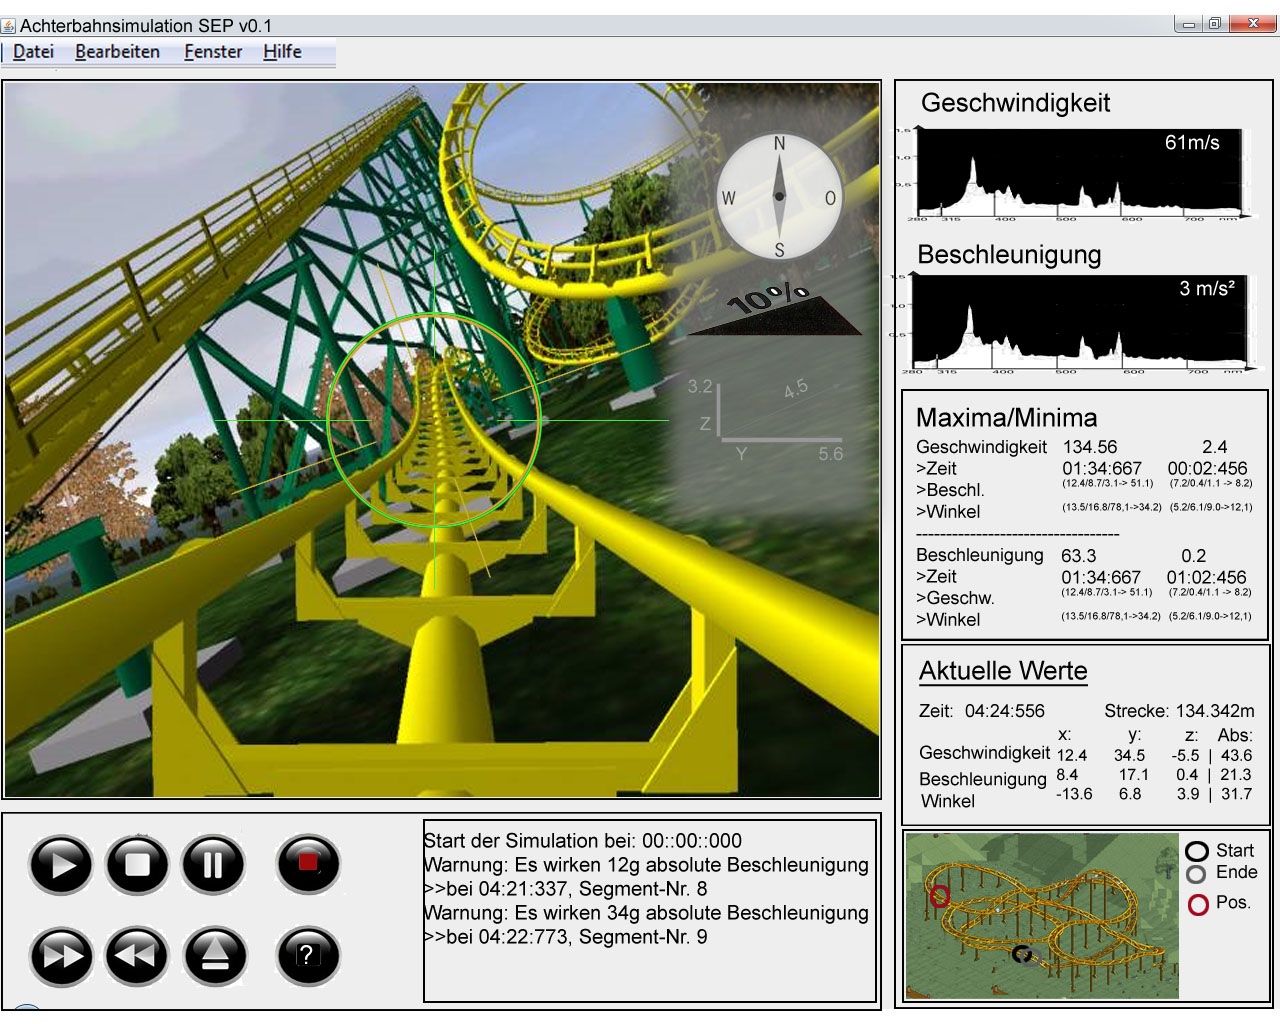
\includegraphics[width=0.8\linewidth]{./bilder/GUI_v2.jpg}%
\caption{Simulation}%
\label{Simulation}%
\end{figure}
%%Beschreibung der Oberfläche und deren Unterteilung
\section*{Simulation}

Die Benutzeroberfläche ist in drei Bereiche unterteilt, die eigentliche Simulation der Achterbahn, eine Anzeige für die Messwerte und ein Bereich für die Steuerung während der Simulation. Die Felder zur Steuerung und Messung können bei Bedarf ein- bzw. ausgeblendet werden.\\
Das Fenster mit den Steuerelementen umfasst Befehle zum Starten, Pausieren, Stoppen und Neustarten der Simulation, sowie\footnote{die folgenden Elemente gehören zu den Wunschkriterien und werden nur umgesetzt, wenn diese innerhalb des Programms berücksichtigt wurden} zur Veränderung der Geschwindigkeit und Aufzeichnung der Simulation als Video.

Das Messfenster beinhaltet ein Diagramm, das die Beschleunigung über die Zeit grafisch aufträgt, die Maximal- und Minimalwerte der Geschwindigkeit und Beschleunigung, die während der Simulation gemessen werden, sowie einen Bereich, in dem die aktuellen Werte von Zeit, Ort, Geschwindigkeit, Beschleunigung und Drehwinkel ausgegeben werden.
Ebenfalls ist eine Minikarte zur Übersicht vorhanden, in der sich ein Abbild der gesamten Achterbahnstrecke mit Start und Ziel, sowie der aktuellen Position des simulierten Wagens markiert werden.

Direkt in dem Simulationsfenster befinden sich Anzeigen zu den wichtigsten Messwerten, wie vertikale und horizontale Beschleunigung, sowie die Drehwinkel um alle drei Raumachsen um das Gefühl der Bewegung zu unterstützen, diese sind bei Bedarf ebenfalls ein-/ausschaltbar. Ebenfalls ist ein Bereich für Hinweise oder Warnungen, die während der Fahrt auftreten können, vorgesehen. 


\section*{Quellenangabe}
Die verwendeten Bilder wurden zwecks Demonstration bearbeitet und arrangiert, die ursprünglichen Quellen sind:
\begin{itemize}
	\item selber erstellt
	\item der Aufgabenbeschreibung entnommen
	\item http://www.leopardgecko.info/Bright-Sun-UV-Desert-Messwerte.jpg
	\item http://hereberobots.com/wp-content/uploads/2010/11/rct002.jpg
	\item http://t1.ftcdn.net/jpg/00/25/12/08/400\_F\_25120801\_ZA9h9NEkaiILe5cJ2jjBPhFXzgZ1aywz.jpg
\end{itemize}       % Kapitel 4
% Kapitel 10
% Die Unterkapitel können auch in separaten Dateien stehen,
% die dann mit dem \include-Befehl eingebunden werden.
%-------------------------------------------------------------------------------

\chapter{Technische Produktumgebung}

\section{Software}
Betriebssystem: Linux.\\
Für die Erstellung und Bearbeitung der Achterbahnspezifikationen gibt es einen Achterbahneditor.\\


\section{Hardware}
Die Software soll auf einem Mittelklasse-PC mit 2 Jahre alter OpenGL-fähiger Grafikkarte laufen.


\section{Orgware}




\section{Produktschnittstellen}
Es existiert bereits ein Achterbahneditor, der die Achterbahnspezifikationen erstellt.//
Der Datenaustausch läuft über eine schematisierte XML-Datei.
           % Kapitel 4
% Kapitel 9
%-------------------------------------------------------------------------------

\chapter{Glossar}
Hier werden Fachbegriffe erklärt.

%------Ende des Dokumentes------------------------------------------------------
\end{document}
